In the previous chapter, we demonstrated how Monte Carlo methods estimate values that would otherwise be difficult to compute directly. The effectiveness of these methods fundamentally depends on our ability to generate random samples from specified probability distributions.

This chapter introduces various techniques for sampling from known target distributions $f(x)$. We assume access to a pseudo-random number generator (RNG)\footnote{For details on RNGs, see Appendix \ref{appendix:rng}.} that produces samples from the continuous uniform distribution $\text{Unif}(0,1)$. Extensions to sampling from unknown distributions are discussed in Chapter \ref{outlook}.

We begin with the inversion method (Section \ref{Inversion Method}), which provides a direct approach when the cumulative distribution function is invertible. Section \ref{box-muller} focuses on generating samples from the Gaussian distribution. Finally, Section \ref{rejection_sampling} introduces techniques for sampling from less tractable distributions through 
rejection sampling methods. 
A variety of other methods are available, including composition, convolution or copula-based methods (see \cite{lemieux_monte_2009}).

\subsection{Inversion Method}
\label{Inversion Method}

The inversion method allows us to sample from any distribution with an invertible cumulative distribution function (CDF). This fundamental technique transforms uniform random variables into samples from the target distribution \citep{murphy_probabilistic_2023, lemieux_monte_2009}.

\begin{theoremrep}[Inverse Transform]
\label{thm:inverse-transform}
Let $U \sim \text{Unif}(0,1)$ and $F$ be an invertible cumulative distribution function. Then $X = F^{-1}(U)$ has distribution function $F$.
\end{theoremrep}

\begin{proof}
For any $x \in \mathbb{R}$:
\begin{align*}
\mathbb{P}(F^{-1}(U) \leq x) 
&= \mathbb{P}(U \leq F(x)) && \text{(applying $F$ to both sides)} \\
&= F(x) && \text{(since $U \sim \text{Unif}(0,1)$)}
\end{align*}
Therefore, $F^{-1}(U)$ has cumulative distribution function $F$. 
\end{proof}

\begin{example}[Exponential Distribution]
\label{ex:exponential-inversion}
To sample from the exponential distribution $\text{Exp}(\lambda)$, we apply the inversion method. The CDF of the exponential distribution is:
$$F(x;\lambda) = 1 - e^{-\lambda x} \quad \text{for } x \geq 0$$

Setting $u = F(x;\lambda)$ and solving for $x$, we obtain the inverse CDF:
$$F^{-1}(u) = -\frac{1}{\lambda}\ln(1-u)$$

Since $U \sim U(0,1)$ implies $1-U \sim U(0,1)$, we can simplify the implementation by using $U$ directly instead of $1-U$.

\begin{algorithm}[H]
\caption{Random Samples from $\text{Exp}(\lambda)$}
\label{algo:exponential-inversion}
\begin{algorithmic}
    \State $U \gets$ \Call{runif\_01}{1} \Comment{Generate uniform random variable}
    \State $X \gets -\frac{1}{\lambda}\ln(U)$ \Comment{Apply inverse transform}
    \State \Return $X$
\end{algorithmic}
\end{algorithm}

\begin{figure}[h]
    \centering
    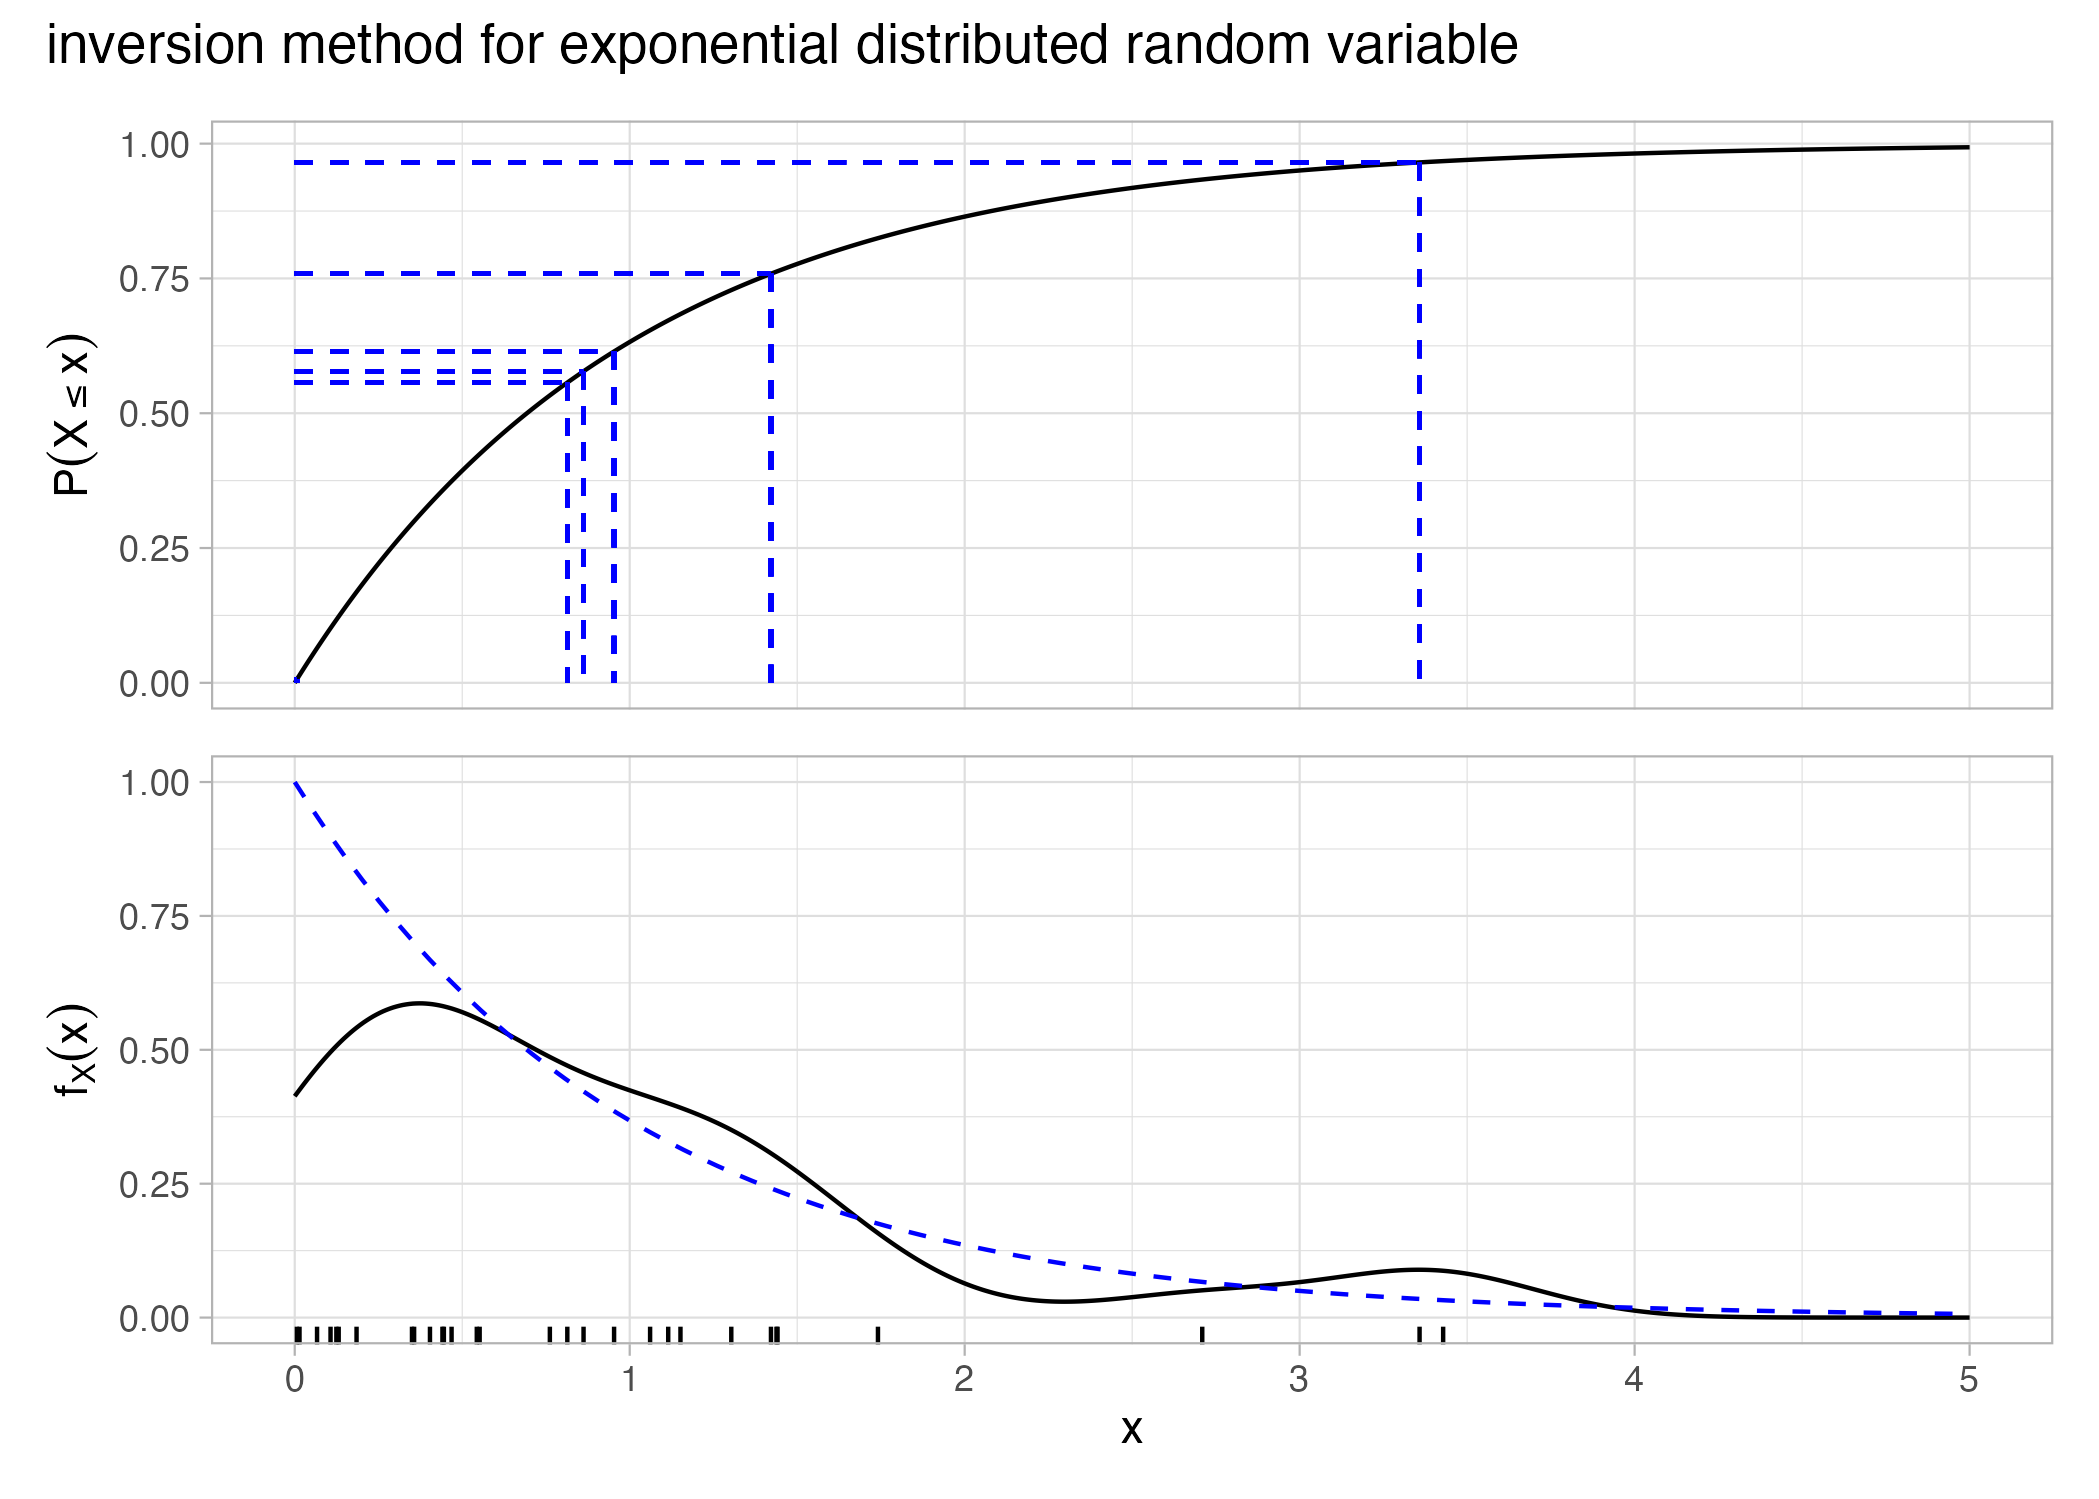
\includegraphics[width=.8\linewidth]{figures/inversion.png}
    \caption{Illustration of the inversion method for generating $\text{Exp}(1)$ random variables. The upper panel demonstrates the transformation process: uniform random samples $U \sim \text{Unif}(0,1)$ are mapped through the inverse cumulative distribution function to yield exponential random variables $X = F^{-1}(U) \sim \text{Exp}(1)$. The lower panel compares the empirical distribution of the generated samples (solid black line) against the theoretical exponential density (dashed blue line), validating the accuracy of the inversion method. Generated using \href{https://github.com/NikoGerman/Seminar/blob/main/Notebooks/inversion-method.Rmd}{\texttt{inversion-method.Rmd}}.}
    \label{fig:inversion-method}
\end{figure}
\end{example}


This demonstrates the power of the inversion method: with a single uniform random variable, we can generate samples from the exponential distribution. Further examples of distributions suitable for the inversion method can be found in \cite{owen_monte_2013}.

\subsection{Box-Muller Method}
\label{box-muller}
The Box-Muller transform is a method for generating pairs of independent standard normal random variables from uniform random variables. The method is based on the polar representation of two independent standard normal variables.

\begin{theoremrep}[Box-Muller Transform]
\label{thm:box-muller}
Let $U_1, U_2 \sim \text{Unif}(0,1)$ be independent uniform random variables. Define:
\begin{equation}
    (X_1, X_2) = \Bigl(\sqrt{-2\ln(U_1)} \cos(2\pi U_2), \sqrt{-2\ln(U_1)} \sin(2\pi U_2)\Bigr)
\end{equation}

Then $X_1, X_2 \sim \mathcal{N}(0,1)$ are independent standard normal random variables.
\end{theoremrep}

\begin{proof}
We prove this by transforming to polar coordinates and applying the change of variables formula.

Let $R = \sqrt{-2\ln(U_1)}$ and $\Theta = 2\pi U_2$. We first determine the joint distribution of $(R, \Theta)$.

\textbf{Step 1: Distribution of $R$.}
Since $U_1 \sim \text{Unif}(0,1)$, we have $-\ln(U_1) \sim \text{Exp}(1)$, which implies $-2\ln(U_1) \sim \text{Exp}(1/2)$. Therefore, $R^2 = -2\ln(U_1) \sim \text{Exp}(1/2)$, making $R$ follow a Rayleigh distribution with parameter 1 (see Appendix \ref{appendix:rayleigh}):
$$f_R(r) = re^{-r^2/2} \quad \text{for } r > 0$$

\textbf{Step 2: Distribution of $\Theta$.}
Since $U_2 \sim \text{Unif}(0,1)$, we have $\Theta = 2\pi U_2 \sim \text{Unif}(0, 2\pi)$ with density:
$$f_\Theta(\theta) = \frac{1}{2\pi} \quad \text{for } \theta \in [0, 2\pi)$$

\textbf{Step 3: Joint distribution of $(R, \Theta)$.}
Since $U_1$ and $U_2$ are independent, $R$ and $\Theta$ are also independent. Therefore:
$$f_{R,\Theta}(r, \theta) = f_R(r) \cdot f_\Theta(\theta) = \frac{r}{2\pi} e^{-r^2/2} \quad \text{for } r > 0, \theta \in [0, 2\pi)$$

\textbf{Step 4: Transformation to Cartesian coordinates.}
The transformation $(X_1, X_2) = (R\cos(\Theta), R\sin(\Theta))$ converts from polar to Cartesian coordinates. The Jacobian matrix is:
$$J = \begin{bmatrix}
\cos(\theta) & -r\sin(\theta) \\
\sin(\theta) & r\cos(\theta)
\end{bmatrix}$$

The determinant is $\det(J) = r\cos^2(\theta) + r\sin^2(\theta) = r$.

\textbf{Step 5: Change of variables.}
Using the change of variables formula (see Appendix \ref{appendix:change_of_vars}), the joint density of $(X_1, X_2)$ is:
\begin{align*}
f_{X_1,X_2}(x_1, x_2) &= f_{R,\Theta}(r, \theta) \cdot \frac{1}{|\det(J)|} \\
&= \frac{r}{2\pi} e^{-r^2/2} \cdot \frac{1}{r} \\
&= \frac{1}{2\pi} e^{-(x_1^2 + x_2^2)/2}
\end{align*}
where we used $r^2 = x_1^2 + x_2^2$.

This joint density factors as:
$$f_{X_1,X_2}(x_1, x_2) = \left(\frac{1}{\sqrt{2\pi}} e^{-x_1^2/2}\right) \cdot \left(\frac{1}{\sqrt{2\pi}} e^{-x_2^2/2}\right)$$

Therefore, $X_1$ and $X_2$ are independent standard normal random variables.
\end{proof}

Algorithm \ref{algo:box-muller} is a simple implementation of the Box-Muller method and produces two independent samples $X_1, X_2 \sim \mathcal{N}(0,1)$, an implementation in \texttt{R} can be found at \href{https://github.com/NikoGerman/Seminar/blob/main/Notebooks/box-muller.Rmd}{\texttt{box-muller.Rmd}}.
\paragraph{Multivariate Normal Random Variables}
To generate multivariate normal random variables, we transform independent standard normal variables using linear transformations.

\begin{theoremrep}[Multivariate Normal Transformation]
\label{thm:multivariate-normal}
Let $Z = (Z_1, \ldots, Z_n)^\top \sim \mathcal{N}_n(\mathbf{0}, I)$ be a vector of i.i.d. standard normal random variables, $\boldsymbol{\mu} = (\mu_1, \ldots, \mu_n)^\top$ be a real-valued mean vector, and $\Sigma \in \mathbb{R}^{n\times n}$ be a symmetric, positive definite covariance matrix. If $L$ is the lower triangular matrix from the Cholesky decomposition\footnote{see Appendix \ref{appendix:Cholesky}.} $\Sigma = LL^\top$, then:
\begin{equation}
    X = \boldsymbol{\mu} + LZ \sim \mathcal{N}_n(\boldsymbol{\mu}, \Sigma)
\end{equation}

\end{theoremrep}

\begin{proof}
We prove this by showing that $X$ has the correct mean and covariance structure.

\textbf{Mean:}
\begin{align*}
\mathbb{E}[X] &= \mathbb{E}[\boldsymbol{\mu} + LZ] \\
&= \mathbb{E}[\boldsymbol{\mu}] + L\mathbb{E}[Z] \\
&= \boldsymbol{\mu} + L \cdot \mathbf{0} = \boldsymbol{\mu}
\end{align*}

\textbf{Covariance:}
\begin{align*}
\text{Cov}(X) &= \text{Cov}(\boldsymbol{\mu} + LZ) \\
&= \text{Cov}(LZ) \\
&= L \cdot \text{Cov}(Z) \cdot L^\top \\
&= L \cdot I_n \cdot L^\top = LL^\top = \Sigma
\end{align*}

Since $X$ is a linear transformation of jointly normal random variables, $X$ is also multivariate normal with mean $\boldsymbol{\mu}$ and covariance $\Sigma$.
\end{proof}

This transformation allows us to generate samples from any multivariate normal distribution using only independent standard normal samples (see Figure \ref{fig:multivariate_normal}).

\begin{figure}[h]
    \centering
    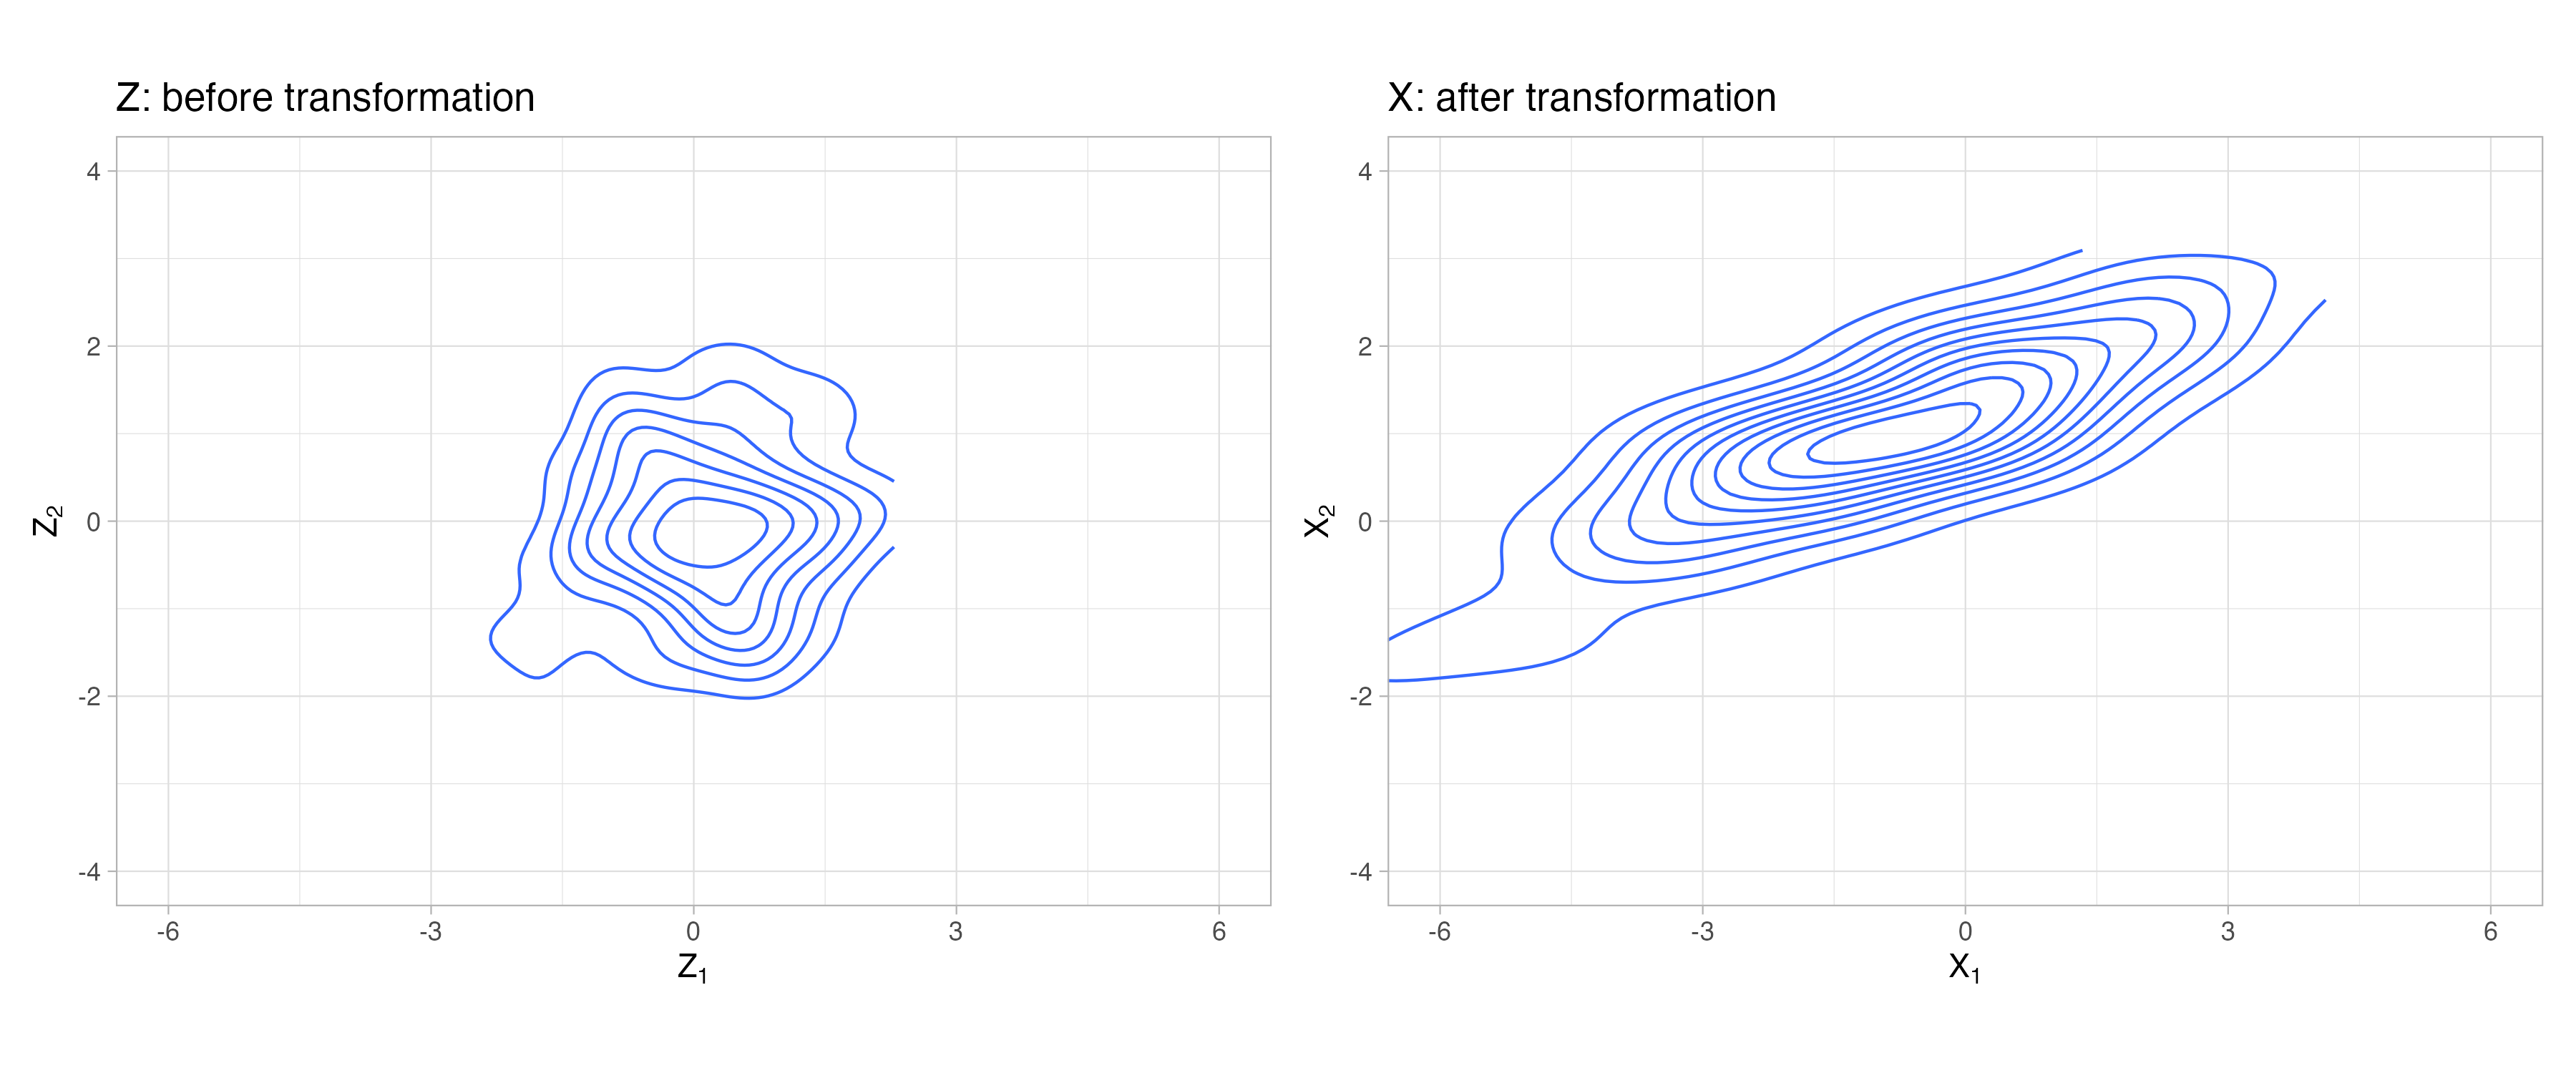
\includegraphics[width=.8\linewidth]{figures/bivariate.png}
    \caption{Visualization of the transformation from standard bivariate normal $\mathcal{N}_2(\boldsymbol{0}, I)$ (left panel) to general bivariate normal $\mathcal{N}_2(\boldsymbol{\mu}, \Sigma)$ (right panel) distributions. The contour plots illustrate the geometric effect of this transformation on the distribution's shape and location. Generated using \href{https://github.com/NikoGerman/Seminar/blob/main/Notebooks/bivariate-normal.Rmd}{\texttt{bivariate-normal.Rmd}}.}
    \label{fig:multivariate_normal}
\end{figure}

\subsection{Acceptance-Rejection}
\label{rejection_sampling}

When the target distribution with density $p(x)$ from which we want to sample is intractable for direct sampling methods (yet somehow easy to evaluate), the \textit{acceptance-rejection} algorithm provides an alternative approach. The idea is to sample from an envelope distribution and then accept or reject these samples according to some criterion. Although this approach wastes some computational effort by throwing away samples, it provides a powerful way to generate samples from complex distributions.

\subsubsection{Basic Rejection Sampling}
Instead of sampling directly from $f(x)$, we sample from $r(x)$, where $r(x)$ is a probability density function and the following envelope condition is satisfied:
\begin{equation*}
    T \cdot r(x) \geq f(x) \quad \forall x
\end{equation*}

We define $t(x) = T \cdot r(x)$. The function $t(x)$ need not be normalized, but must satisfy the condition $T = \int t(x)dx < \infty$.

The acceptance-rejection algorithm can be characterized as follows:
\begin{enumerate}
    \item Generate a candidate $\tilde{X} \sim r$
    \item Generate $U \sim \text{Unif}(0,1)$ independent of $\tilde{X}$
    \item If $U \leq \frac{f(\tilde{X})}{t(\tilde{X})}$, accept and set $X = \tilde{X}$; otherwise, reject and return to step 1.
\end{enumerate}

\begin{theoremrep}[Acceptance-Rejection Sampling]
Let $X$ denote an accepted sample. Then $X$ has cumulative distribution function $F(x) = \int_{-\infty}^x f(y)dy$.
\end{theoremrep}

\begin{proof}
We need to show that 
$$\mathbb{P}(X \leq x) = \mathbb{P}\left(\tilde{X} \leq x \mid U \leq \frac{f(\tilde{X})}{t(\tilde{X})}\right) = F(x)$$

Using the definition of conditional probability:
\begin{align*}
    \mathbb{P}\left(\tilde{X} \leq x \mid U \leq \frac{f(\tilde{X})}{t(\tilde{X})}\right) &= \frac{
    \mathbb{P}\left(\tilde{X} \leq x, U \leq \frac{f(\tilde{X})}{t(\tilde{X})}\right)}{\mathbb{P}\left(U \leq \frac{f(\tilde{X})}{t(\tilde{X})}\right)}
\end{align*}

For the numerator, using the law of total probability and independence of $U$ and $\tilde{X}$:
\begin{align*}
    \mathbb{P}\left(\tilde{X} \leq x, U \leq \frac{f(\tilde{X})}{t(\tilde{X})}\right) &= \int_{-\infty}^x \mathbb{P}\left(U \leq \frac{f(y)}{t(y)}\right) r(y) dy \\
    &= \int_{-\infty}^x \frac{f(y)}{t(y)} r(y) dy \\
    &= \frac{1}{T}\int_{-\infty}^x f(y) dy
\end{align*}

For the denominator:
\begin{align*}
    \mathbb{P}\left(U \leq \frac{f(\tilde{X})}{t(\tilde{X})}\right) &= \int_{-\infty}^{\infty} \frac{f(y)}{t(y)} r(y) dy \\
    &= \frac{1}{T}\int_{-\infty}^{\infty} f(y) dy = \frac{1}{T}
\end{align*}

Therefore:
\begin{align*}
    \mathbb{P}\left(\tilde{X} \leq x \mid U \leq \frac{f(\tilde{X})}{t(\tilde{X})}\right) &= \frac{\frac{1}{T}\int_{-\infty}^x f(y) dy}{\frac{1}{T}} = \int_{-\infty}^x f(y) dy = F(x)
\end{align*}
\end{proof}

The implementation of acceptance-rejection is straight-forward (see Algorithm \ref{algo:acceptance-rejection}). The main challenge is sampling from $r(x)$ and possibly the evaluation of $f(\cdot)$ and $t(\cdot)$. For the former challenge we assume to have access to some algorithm \texttt{rand\_r()}, which samples from $r(x)$.

\subsubsection{Adaptive Rejection Sampling}
Adaptive rejection sampling is an extension of the basic acceptance-rejection method that automatically constructs and refines the envelope function during the sampling process. For log-concave target densities, the algorithm exploits the property that tangent lines to the log-density provide a tight upper bound. The method begins with an initial set of tangent points and iteratively improves the piecewise-linear envelope by adding new tangent lines at rejected sample locations. Algorithm \ref{algo:adaptive-rejection} demonstrates a basic implementation. 

The adaptive refinement ensures that the envelope becomes increasingly efficient over time, dramatically reducing the rejection rate as more samples are drawn. For more detailed information on adaptive rejection sampling, see \cite{murphy_probabilistic_2023}.
